\section{Windows GUI}
I dette afsnit beskrives designet af Windows applikationen. I Windows applikationen designes view-klasser, der implementerer view-interfacet defineret i præsentationslaget. De dominante user interface frameworks på Windows kaldes .NET og WPF, hvor der her bruges WPF, som er en overbygning på .NET. 
Designet af Windows GUI er lavet således, at codebehind filerne implementerer hver sit view-interfacet fra præsentationslaget.
Codebehind agerer dermed bro i mellem Smartpools præsentationslag og WPF view-lag.

I klasse diagrammet nedenfor, ses Windows designet, med de klasser der implementerer view-interfaces.
\begin{landscape}
\begin{figure}
\centering
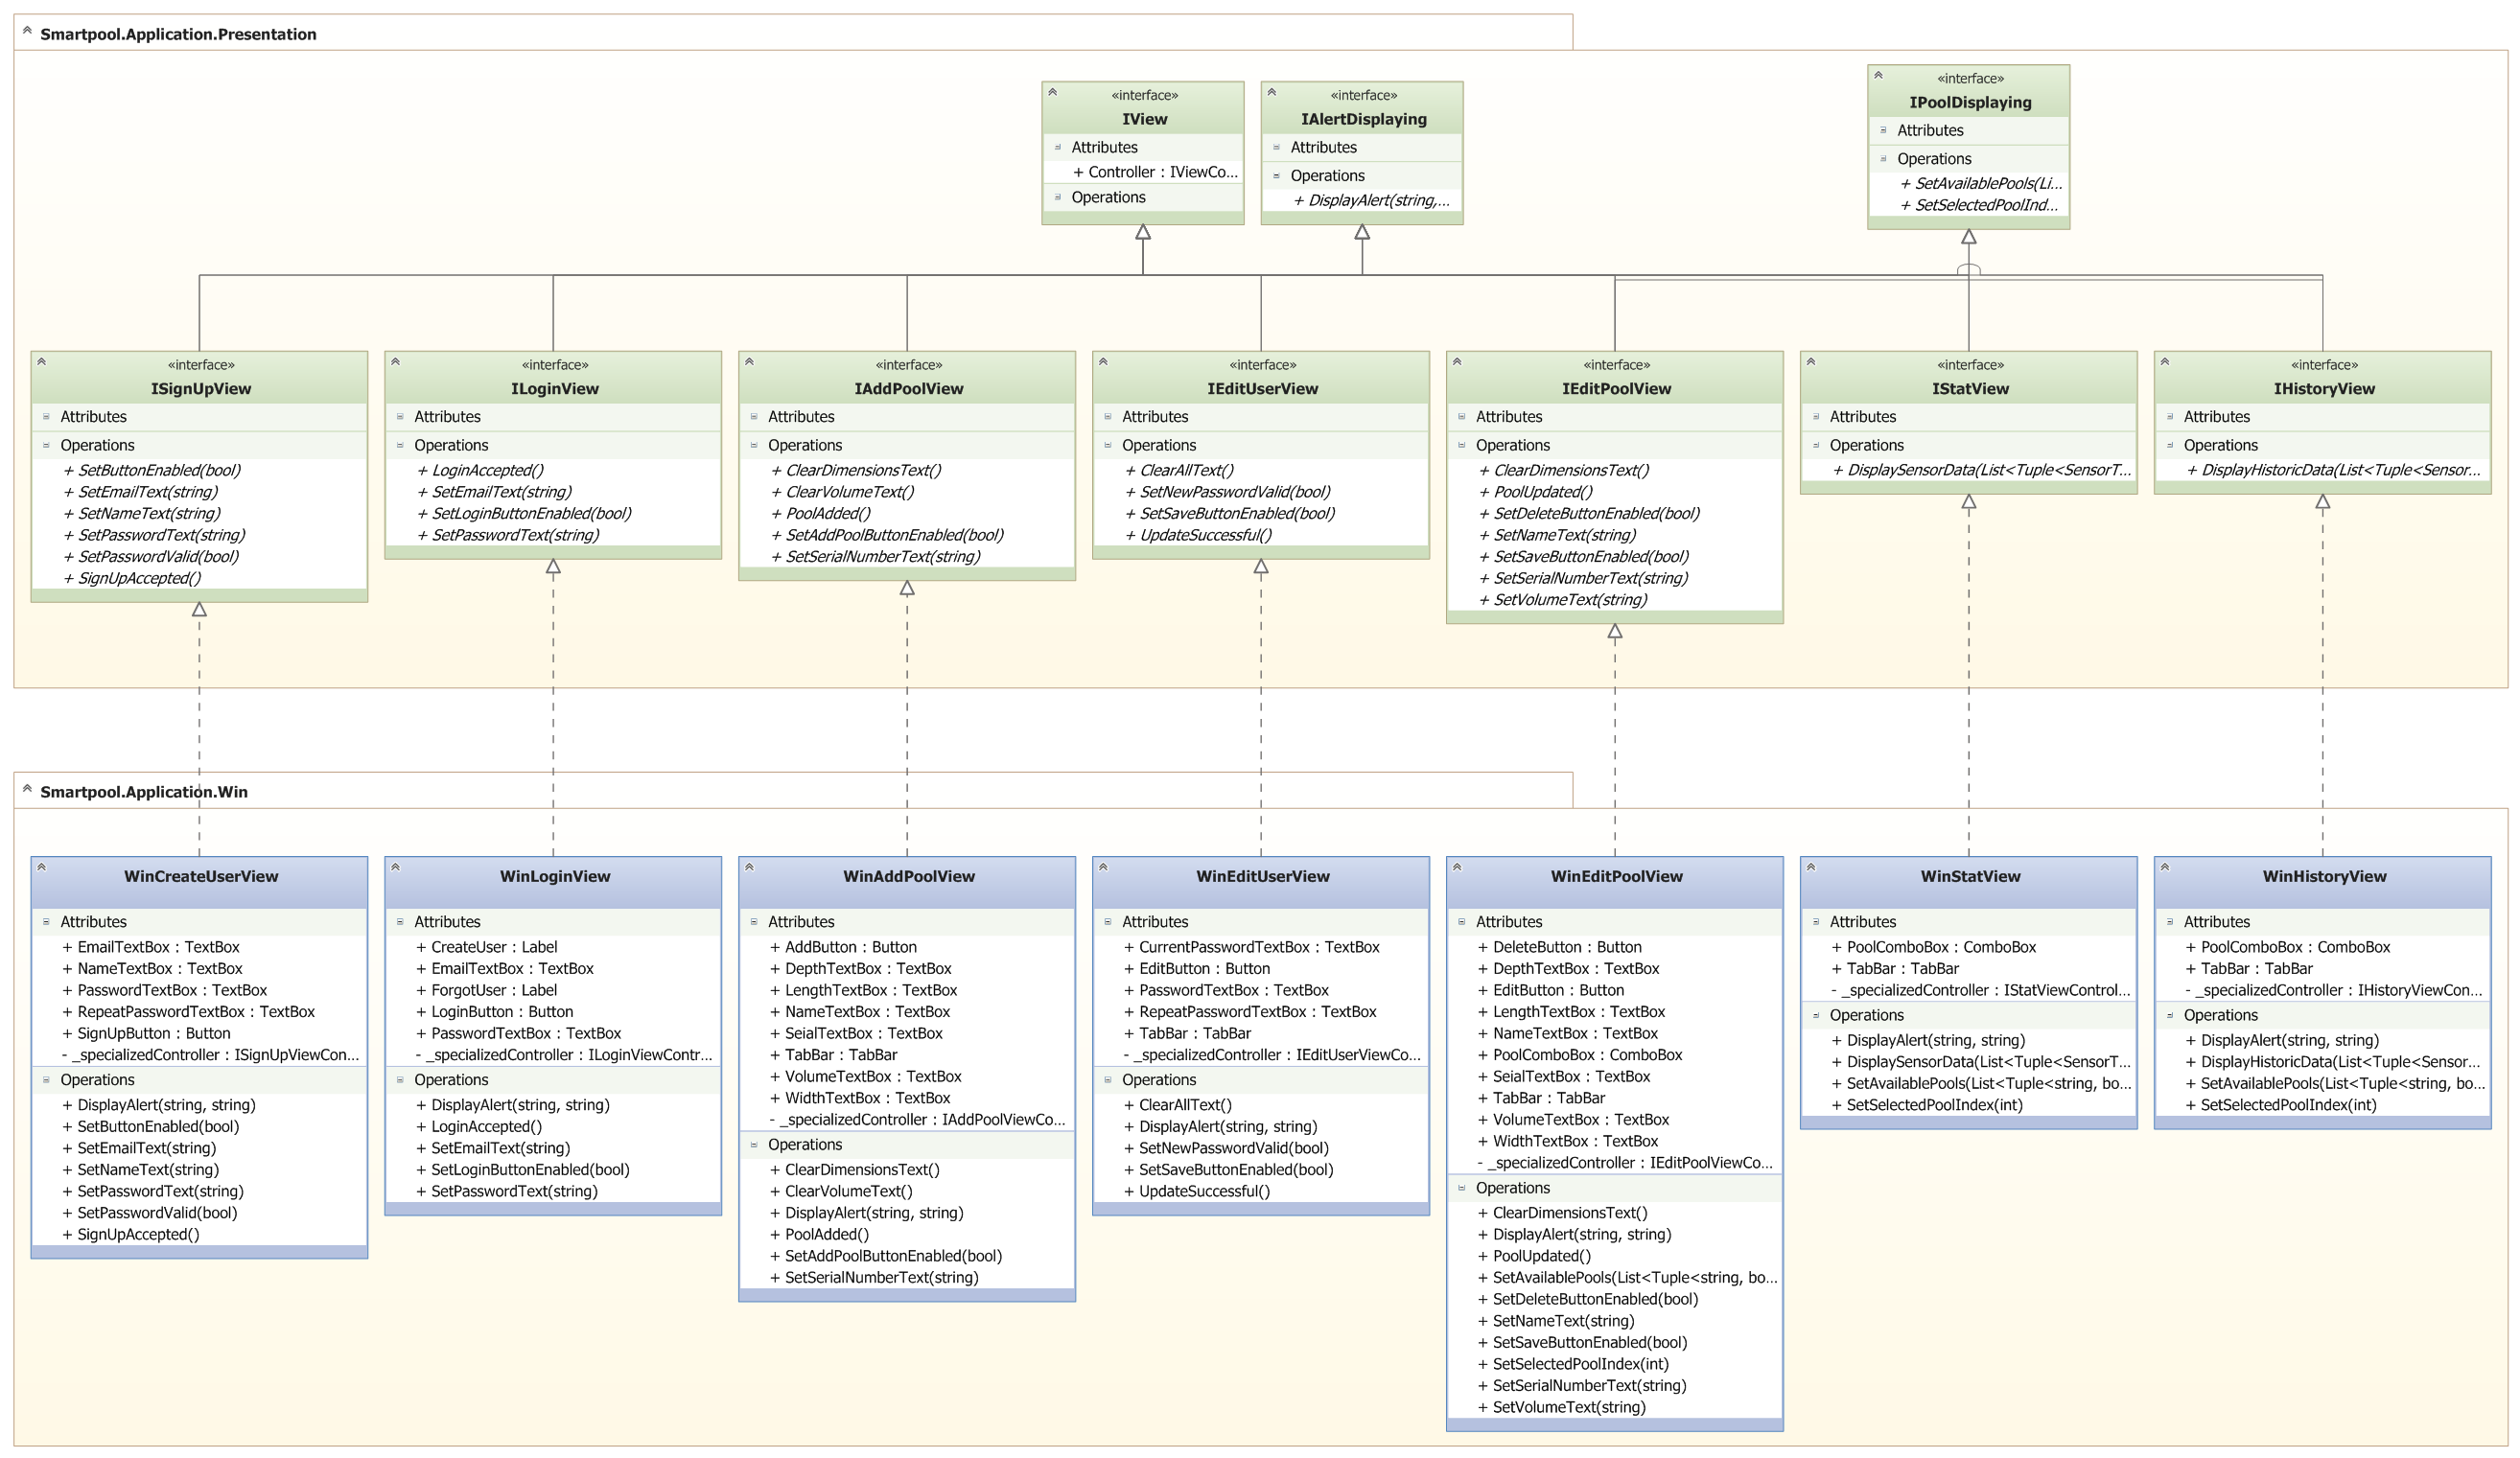
\includegraphics[width=1\linewidth]{figs/design/win_uml_full}
\caption{Fuldt klassediagram for Windows applikation}
\label{fig:win_uml_full}
\end{figure}
\end{landscape}

Af klassediagrammet fremgår det, at alle WPF klasserne har en "\_specializedController" property. Denne property, der bør typecaste sin nedarvede IViewController property, til den type presenter, der passer specifikt til view'et.

\subsection{Klassedesign}
I dette afsnit beskrives designet af de enkelte view-implementerende klasser i Smartpool.Application.Win. Hver klasse, der beskrives i dette afsnit er en WPF codebehind klasse, der implementerer et view-interface defineret i Smartpools præsentationslag.

\subsubsection{WinCreateUserView}
WinCreateUserView-klassen implementerer ISignUpView interfacet. Klassen indeholder en række WPF/.NET user interface elementer, som passer sammen med klasse interfacet. Da dette view omhandler brugeroprettelse, er klassen designet til at indeholde en række tekstfelter, og en knap til at fuldende brugeroprettelsen. 

\subsubsection{WinLoginView}
WinLoginView-klassen implementerer ILoginView interfacet. Da dette view håndterer login, er klassen designet til at indeholde to tekstfelter, og en knap til at godkende login.

\subsubsection{WinAddPoolView}
WinAddPoolView-klassen implementerer IAddPoolView interfacet. Klassen indeholder en række WPF/.NET user interface elementer, som tekstfelter og en knap, der passer sammen med metoderne i interfacet. 

\subsubsection{WinEditUserView}
WinEditUserView-klassen implementerer IEditUserView interfacet. Klassen indeholder en række WPF/.NET user interface elementer, som tekstfelter og en knap, der passer sammen med metoderne i interfacet.

\subsubsection{WinEditPoolView}
WinEditPoolView-klassen implementerer IEditPoolView interfacet. Da dette view håndterer redigering af pools, indeholder klassen tekstfelter, og knap til at foretage ændringer eller slette en pool. 
Klassen indeholder også en PoolComboBox, som type knap med en liste, der er tænkt at skulle bruges til skift imellem pools i systemet. Denne knap er tilføjet klassen, da IEditPoolView interfacet implementerer IPoolDisplaying interfacet.

\subsubsection{WinStatView}
WinStatView-klassen implementerer IStatView interfacet. Dette view håndterer dynamisk visning af nyeste måledata.
Klassen indeholder også en PoolComboBox, som type knap med en liste, der er tænkt at skulle bruges til skift imellem pools i systemet. Denne knap er tilføjet klassen, da IEditPoolView interfacet implementerer IPoolDisplaying interfacet.

\subsubsection{WinHistoryView}
WinHistoryView-klassen implementerer IHistoryView interfacet. Dette view håndterer dynamisk visning af historisk måledata.
Klassen indeholder også en PoolComboBox, som type knap med en liste, der er tænkt at skulle bruges til skift imellem pools i systemet. Denne knap er tilføjet klassen, da IEditPoolView interfacet implementerer IPoolDisplaying interfacet. 